\chapter{Cloud Computing}
Cloud computing is a model for enabling ubiquitous, convenient, on-demand network access to a shared pool of configurable computing resources that can be rapidly provisioned and released with minimal management effort or service provider interaction.
This cloud model is composed of five \textbf{essential characteristics:}
\begin{itemize}
    \item On-demand self service
    \item Measured service
    \item Broad network access
    \item Rapid elasticity
    \item Resource pooling
\end{itemize}
It is composed of \textbf{three service models:}
\begin{itemize}
    \item  Software as a service \textbf{(SAAS)}
    \item Platform as a service \textbf{(PAAS)}
    \item Infrastructure as a service \textbf{(IAAS)}
\end{itemize}
And finally it is composed by \textbf{four deployment models:}
\begin{itemize}
    \item \textit{Public} cloud
    \item \textit{Private} cloud
    \item \textit{Hybrid} cloud
    \item \textit{Community} cloud
\end{itemize}

Cloud computing is a specialized form of \textbf{distributed computing} that introduces utilization model for remotely provisioning scalable and measured resources.

One possible error that can be made is to confuse \textit{cloud computing} and \textit{data center} concepts
\begin{itemize}
    \item \textbf{Cloud Computing} has the goal of providing services
    \item \textbf{Data Center} can be considered only as a collection of a large amount of data stores to provide data
\end{itemize}

\section{Terminology}
\begin{itemize}
    \item \textbf{Cluster of workstation:} a cluster is a group of independent IT resources that are interconnected and work as a single system.
    \item \textbf{Grid computing:} a computing grid provides a platform in which computing resources are organized into one or more logical pools. Grid computing systems can involve computing resources that are heterogeneous and geographically dispersed, which is generally not possible with cluster computing-based systems. Grid computing is based on a middleware layer that is deployed on computing resources. This middle tier can contain load balancing logic, fail over controls, and autonomic configuration management, each having previously inspired similar cloud computing technologies.
    \item \textbf{Virtualization:} Virtualization represents a technology platform used for the creation of virtual instances of IT resources. These resources can be shared by a set of users. Modern virtualization improves performance reliability and scalability.
    \item \textbf{Distributed computing:} tightly coupled, homogeneous and single administration
    \item \textbf{Cloud Computing:} On demand, service guarantee, virtualization
    \item \textbf{Enabling cloud computing technologies:} Other areas of technology continue to contribute on the modern cloud-based platforms, these are distinguished as \textit{cloud-enabling technologies:}
    \begin{itemize}
        \item Broadband Networks and Internet Architecture
        \item Data Center Technology
        \item Virtualization Technology
        \item Web Technology
        \item Service Technology
    \end{itemize}
\end{itemize}

\section{Motivations}
\begin{itemize}
    \item \textbf{Scalability needs:} there’s the need of passing from a single PC to a data center because of the exponential growing of data and users
    \item \textbf{Computational needs:}  there’s the need of extend the computing power adding many servers because of the increase of web pages, images, users and queries on the net.
\end{itemize}

\section{Definition}
The \textbf{fundamental concepts} belonging to the notion of cloud computing are the following one.
\subsection{Cloud}
A cloud refers to a distinct environment that is designed for the purpose of remotely provisioning scalable and measured resources.
\begin{itemize}
    \item As a specific environment, a cloud has a finite \textit{boundary}
    \item Resources provided by cloud environments are dedicated to supplying back-end processing capabilities and user-based access to these capabilities
\end{itemize}

\subsection{IT resource}
An IT resource is a \textit{physical} or \textit{virtual} IT-related \textbf{artifact} that can be either \textit{software-based}, such as a virtual server or a custom software program, or \textit{hardware-based}, such as a physical server or a network device.

\subsection{Cloud Consumers and Cloud Providers}
\begin{itemize}
    \item The party that provides cloud-based IT resources is the \textit{cloud provider}
    \item The party that uses cloud-based IT resources is the \textit{cloud consumer}
\end{itemize}

\subsection{Scaling}
Scaling represents the \textbf{ability of the IT resource to handle increased or decreased usage} demands. And there are two types:
\begin{itemize}
    \item \textbf{Horizontal Scaling:} is referred to the allocating or releasing of IT resources that are of the same type.
    \begin{itemize}
        \item The horizontal \textit{allocation} of resources is referred to as \textbf{scaling out}
        \item The horizontal \textit{releasing} of resources is referred to as \textbf{scaling in}
    \end{itemize}
    An example of Horizontal scaling can be seen in the following image where an IT resource (Virtual Server A) is scaled out by adding more of the same IT resources (Virtual Servers B and C).

\begin{figure}[!h]
    \centering
    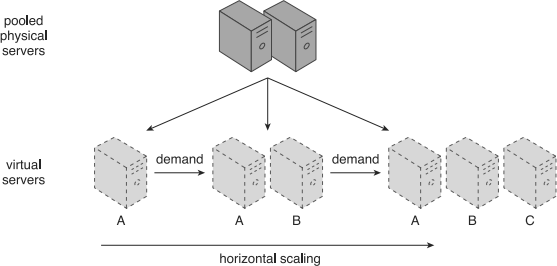
\includegraphics[width=.60\linewidth]{images/CloudComputing/HorizontalScaling.png}
    \caption{Example of Horizontal scaling}
\end{figure}
    
    \item \textbf{Vertical Scaling:} when an existing IT resource is \textit{replaced by another} with higher or lower capacity, vertical scaling is considered to have occurred.
    \begin{itemize}
        \item The replacing of an IT resource with another that has a \textit{higher capacity} is referred to as \textbf{scaling up}
        \item The replacing an IT resource with another that has a \textit{lower capacity} is considered \textbf{scaling down}
    \end{itemize}
    An example of Vertical scaling can be seen in the following image, where an IT resource (a virtual server with two CPUs) is scaled up by replacing it with a more powerful IT resource with increased capacity for data storage (a physical server with four CPUs)
    
\begin{figure}[!h]
    \centering
    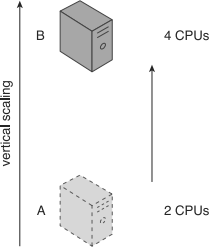
\includegraphics[width=.30\linewidth]{images/CloudComputing/VerticalScaling.png}
    \caption{Example of Vertical scaling}
\end{figure}
\end{itemize}


\section{Cloud Service}
A \textbf{cloud service} is any IT resource that is made \textit{remotely accessible} via a cloud. A Cloud Service could be:
\begin{itemize}
    \item A service with a published technical interface accessed by a consumer outside of the cloud which is likely being invoked by a consumer program
    \item A service that exists as a virtual server is also being accessed from outside of the cloud’s boundary, like by a human user that has remotely logged on to the virtual server
\end{itemize}
The \textbf{cloud service consumer} is a temporary runtime role assumed by a software program when it accesses a cloud service.

\section{Cloud Computing Advantages}
\begin{itemize}
    \item \textbf{Performance}
    \item \textbf{Cost reduction:} the number of investments is reduced and there’s an access to powerful infrastructures without purchasing them. More benefits like:
    \begin{itemize}
        \item On-demand access to pay-as-you-go computing resources
        \item The perception of having unlimited computing resources that are available on demand
        \item The ability to add or remove IT resources at a fine-grained level
    \end{itemize}
    \item \textbf{Scalability:} clouds can instantly and dynamically allocate IT resources to cloud consumers, on-demand or via the cloud consumer’s direct configuration
    \item \textbf{Availability} and \textbf{Reliability:} cloud environment provides an extensive support for increasing the \textit{availability} of a cloud-based IT resource to minimize or even eliminate outages. And for increasing its \textit{reliability} so as to minimize the impact of runtime failure conditions
    \item Maximize resource utilization
\end{itemize}  

\section{Risk and Limits}
Cloud computing can introduce distinct risks and limits that should be considered when we want to use it. In particular:
\begin{itemize}
    \item Requires high and available connection between nodes
    \item Introduce security problems like authentication on the usage of shared resources and private resources
    \item Lack of industry standard, public cloud are usually proprietary
    \item Limited portability between cloud providers
\end{itemize}

\section{Cloud Delivery Models}
A cloud delivery model represents a specific, pre-packaged combination of IT resources offered by a cloud provider. It refers to the types of services offered by cloud computing. Three common cloud delivery models have become widely established and formalized:
\subsection{Infrastructure as a Service (IaaS)} 
    \begin{itemize}
        \item \textbf{Cloud Provider} offers access to fully functioning software
        \item \textbf{Service Provider} owns the equipment and is responsible for housing, running and maintaining it
        \item \textbf{Client} typically pays on a per-use basis
        \item The main \textbf{goal} of IaaS environment is to provide cloud consumers with a high level of control and responsibility over its configuration and utilization
        \item The resources provided by IaaS are not preconfigured therefore this model is used by cloud consumers that require a high level of control over the cloud enviroment
        \item \textbf{Examples:} Amazon Web Services, Google Cloud Storage, DigitalOcean.
    \end{itemize}
    
\begin{figure}[!h]
    \centering
    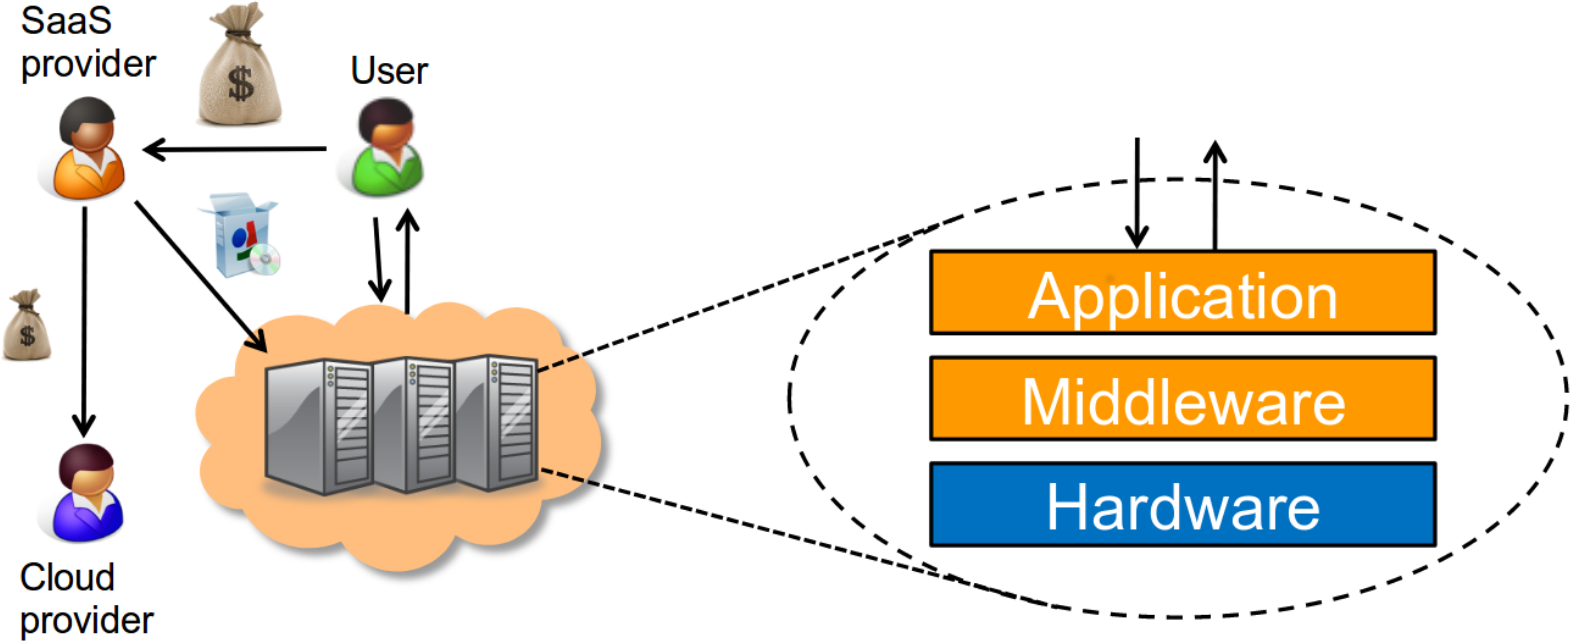
\includegraphics[width=.60\linewidth]{images/CloudComputing/iaas.png}
    \caption{Infrastructure as a Service structure}
\end{figure}

\subsection{Platform as a Service (PaaS)}
\begin{itemize}
    \item The \textbf{cloud provider} give the way to rent hardware, operating systems, storage
    \item The \textbf{service delivery model} allows the customer to rent virtualized servers and associated services for running existing applications or developing and testing new ones
    \item The \textbf{service provider} offers a complete platform solution thatthe user runs software on
    \item The \textbf{platform} usually consists of an operating system and an execution environment
    \item  In this model, customers \textbf{don’t want to think about the server} or its internals, they want to point to a virtual machine
    \item  It is a \textbf{’ready to use’} environment with IT resources already deployed and configured
    \item \textbf{Examples:} Windows Azure, Google App Engine, Heroku
\end{itemize}

\begin{figure}[!h]
    \centering
    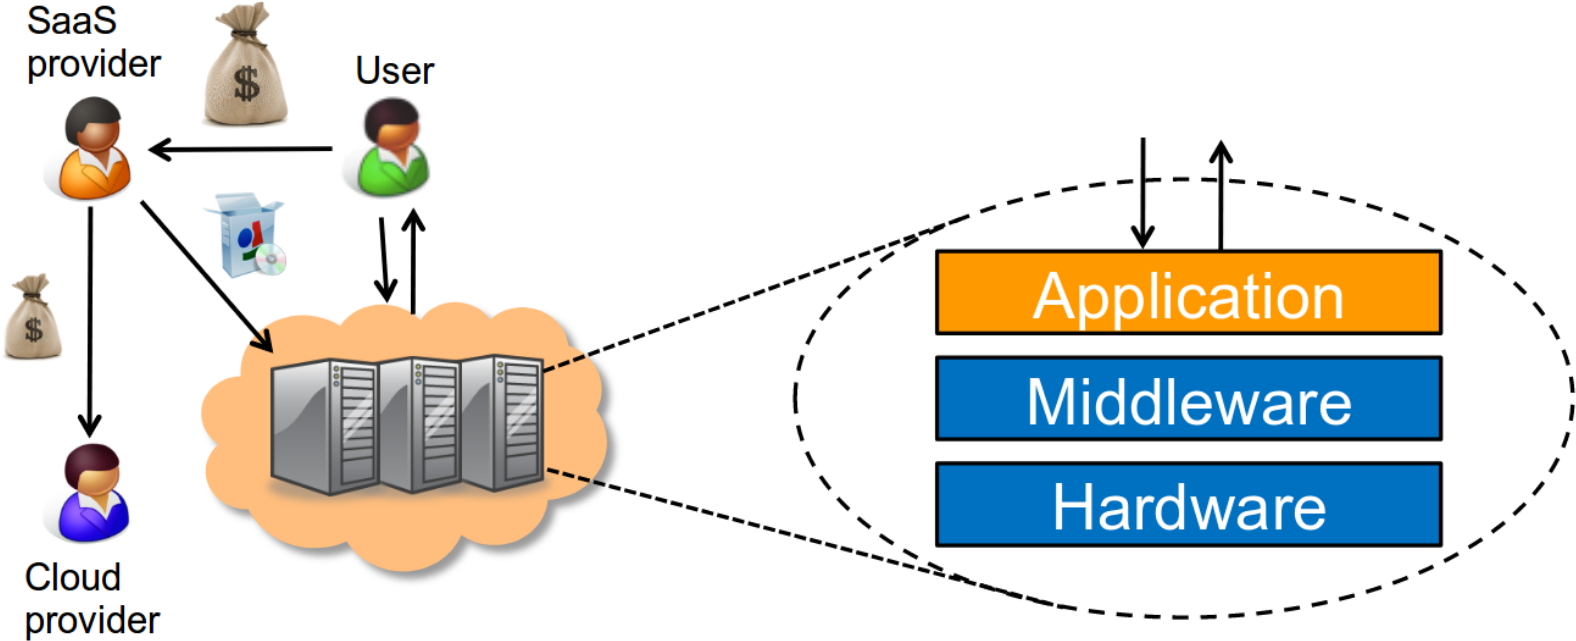
\includegraphics[width=.60\linewidth]{images/CloudComputing/paas.png}
    \caption{Platform as a Service structure}
\end{figure}

\subsection{Software as a Service (SaaS)}
\begin{itemize}
    \item The \textbf{cloud provided} rents applications software, that are hosted by the \textit{provider} in the cloud and it is available to \textit{customers} over a network
    \item The \textbf{user} rents access to a physical or virtual server
    \item The \textbf{user} has full control and responsibility over the running operating system and can use it to run any software
    \item \textbf{Examples:} Google Apps, Yahoo!Mail, CRM software.
\end{itemize}

\begin{figure}[!h]
    \centering
    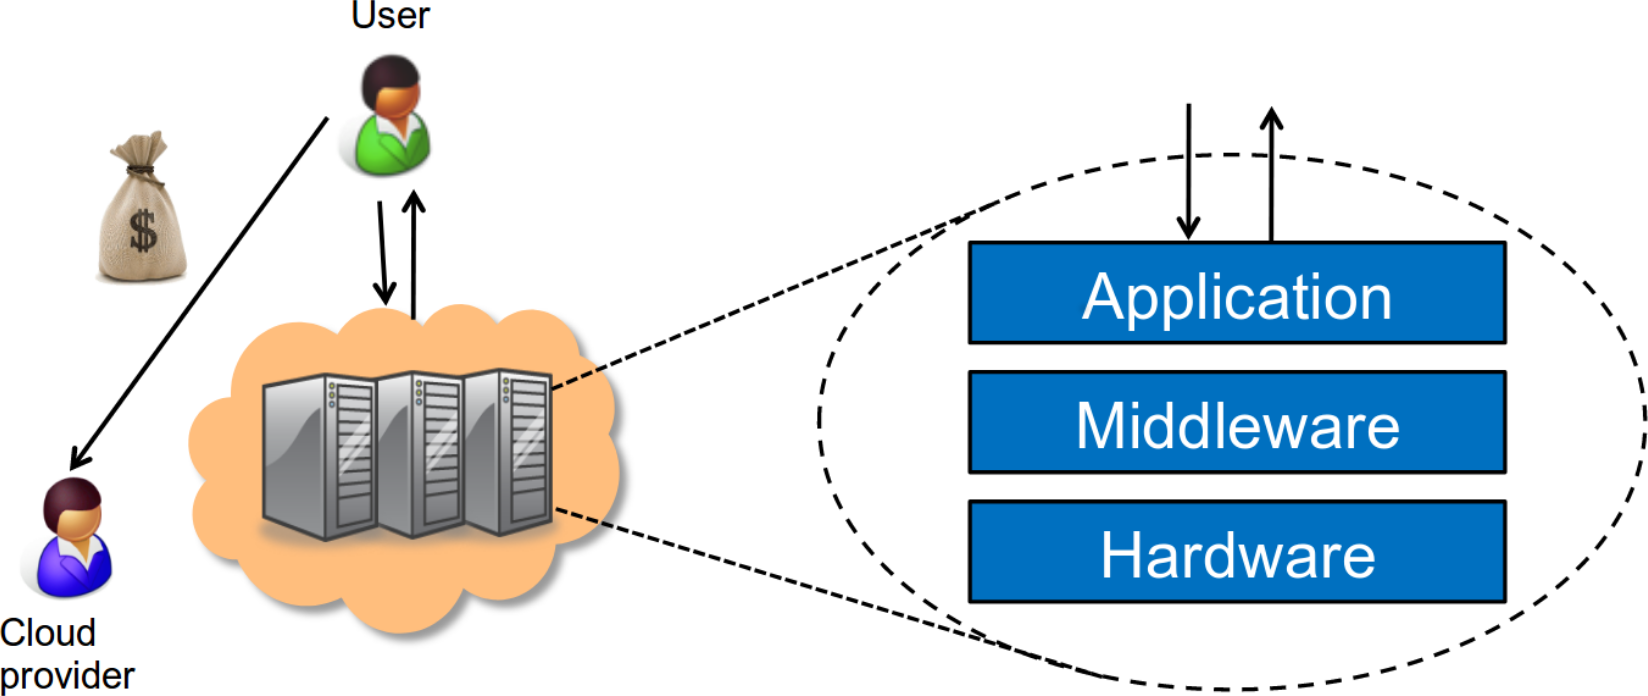
\includegraphics[width=.60\linewidth]{images/CloudComputing/saas.png}
    \caption{Software as a Service structure}
\end{figure}

\section{Cloud Deployment Models}
Cloud deployment model defines a specific type of cloud environment primarily distinguished by ownership, size and access.
\begin{itemize}
    \item \textbf{Public Cloud:} the \textit{owner} is the cloud provider and \textit{services} are accessible for everyone
    \item \textbf{Community Cloud:} the \textit{owner} is a community of consumers and it customers outside of it are not granted to access and use services and resources.  A community cloud is similar to a public cloud except that its access is limited to a specific community of cloud consumers.
    \item \textbf{Private Cloud:} the \textit{owner} is a single organization and only its \textit{customers} can access to services and resources. It enables an organization to use cloud computing technology as a means of centralizing access to IT resources by different locations
    \item \textbf{Hybrid Cloud:} formed most commonly by \textit{private} and \textit{public} cloud. Usually cloud consumer choose to deploy cloud services processing \textbf{sensitive data} to a \textit{private cloud} and \textbf{less sensitive} cloud services to a \textit{public cloud}
\end{itemize}

\section{Potentialities and concerns}
\begin{itemize}
    \item \textbf{Why use a cloud computing system?} For its advantages: cost, scalability and performance
    \item \textbf{Cases where cloud computing system cannot be adopted:} legislative frameworks, medical records and data privacy
\end{itemize}